\documentclass[a4paper, 12pt]{article}%тип документа

%отступы
\usepackage[left=0.6cm,right=1cm,top=2cm,bottom=3cm,bindingoffset=0cm]{geometry}
\setlength{\parindent}{5ex}

%Русский язык
\usepackage[T2A]{fontenc} %кодировка
\usepackage[utf8]{inputenc} %кодировка исходного кода
\usepackage[english,russian]{babel} %локализация и переносы

%Вставка картинок
\usepackage{graphicx}
\graphicspath{{pictures/}}
\DeclareGraphicsExtensions{.pdf,.png,.jpg}

%Графики
\usepackage{pgfplots}
\pgfplotsset{compat=1.9}

%Математика
\usepackage{amsmath, amsfonts, amssymb, amsthm, mathtools}

%Таблицы
\usepackage{longtable} 
\usepackage{float}

%Римские цифры
\newcommand{\RomanNumeralCaps}[1]{\uppercase\expandafter{\romannumeral#1}}

\usepackage{multirow}


\begin{document}
	\begin{titlepage}
		\begin{center}
			\textsc{Федеральное государственное автономное образовательное учреждение высшего образования«Московский физико-технический институт (национальный исследовательский университет)»\\[5mm]
			}
			
			\vfill
			
			\textbf{Отчёт по лабораторной работы 4.4.2 \\[3mm]
				ИЗУЧЕНИЕ ФАЗОВОЙ РЕШЕТКИ (ЭШЕЛЕТ)
				\\[50mm]
			}
			
		\end{center}
		
		\hfill
		\begin{minipage}{.5\textwidth}
			Выполнил студент:\\[2mm]
			Сериков Алексей Романович\\[2mm]
			группа: Б03-103\\[5mm]
			
		\end{minipage}
		\vfill
		\begin{center}
			Москва, 2023 г.
		\end{center}
		
	\end{titlepage}
	
	\newpage
	\textbf{Аннотация}\\
	
	
	\textbf{Цель работы: }\\
	
	Знакомство с работой гониометра и определение спектральных характеристик фазовой решётки (эшелета).
	
	\textbf{В работе используются: }\\
	
	Ртутная лампа, гониометр, амплитудная и фазовая дифракционные решётки, плоскопараллельная стеклянная пластинка, призменный уголковый отражатель, щель с микрометрическим винтом.
	\\
	
	
	
	\textbf{Теория:}
	
	
Дифракционная решётка представляет собой стеклянную или металлическую пластину, на которую через строго одинаковые интервалы нанесены параллельные штрихи. Основные параметры дифракционной решётки "--- период $d$ (постоянная решётки), число штрихов $N$.
Условие дифракции Фраунгофера "--- решётка освещается плоской волной, а плоскость наблюдения практически находится в бесконечности.

	\begin{figure}[H]
	\begin{center}
		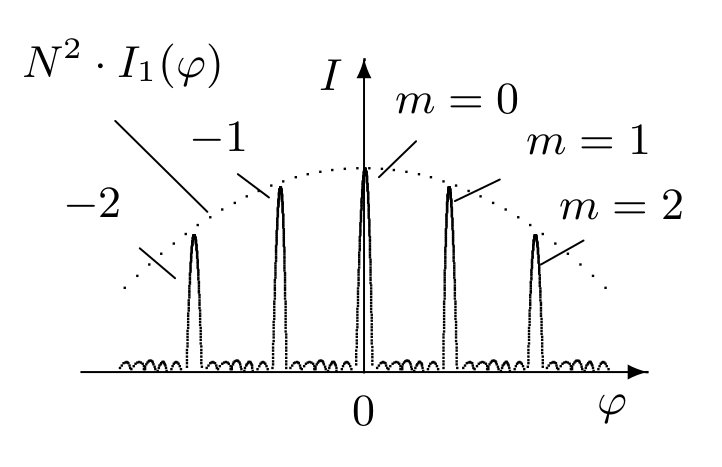
\includegraphics[width=0.6\linewidth]{1.png}
		\caption{Распределение интенсивности света при дифракции Фраунгофера на решётке}
	\end{center}
\end{figure}
	
	
	
Согласно принципу Гюйгенса-Френеля распределение интенсивности в дифракционной картине определяется суперпозицией волн; амплитуды всех интерферирующих волн при $\varphi$ практически одинаковы; фазы составляют арифметическую прогрессию:
\begin{equation}
	d \sin \varphi_m = m \lambda,
\end{equation}

где $m \in Z$ "--- порядок спектра.
	
	Интенсивность $I$ света, распространяющегося под углом $\varphi$ к нормали:
\begin{equation}
	I = I_1(\varphi)\frac{\sin^2 (N(dk \sin \varphi) / 2)}{\sin^2 ((dk \sin \varphi) 2)},
\end{equation}
	где $k = \frac{2 \pi}{\lambda}$ "--- волновое число.
	
	Дисперсия $D$ характеризует угловое расстояние между близкими спектральными линиями:
\begin{equation}
	D = \frac{d \varphi}{d \lambda} = \frac{m}{d \cos \varphi} = \frac{m}{\sqrt{d^2 - m^2 \lambda^2}}
\end{equation}
	Согласно критерию разрешения Релея, линии становятся неразличимыми, когда расстояние между ними меньше, чем расстояние от максимума одной линии до её первого минимума:
\begin{equation}
	\frac{Nkd}{2}(\sin (\varphi + \Delta \varphi) - \sin \varphi) = \pi,
\end{equation}
	где $\Delta \varphi$ "--- угловая полуширина главного максимума, $\Delta \varphi = \frac{\lambda}{Nd \cos \varphi}$
	
	
	Разрешающая способность спектрального прибора $R$ вычисляется по формуле:
\begin{equation}
	R = \frac{\lambda}{\Delta \lambda} = m \cdot N
\end{equation}
	\begin{figure}[H]
		\begin{center}
			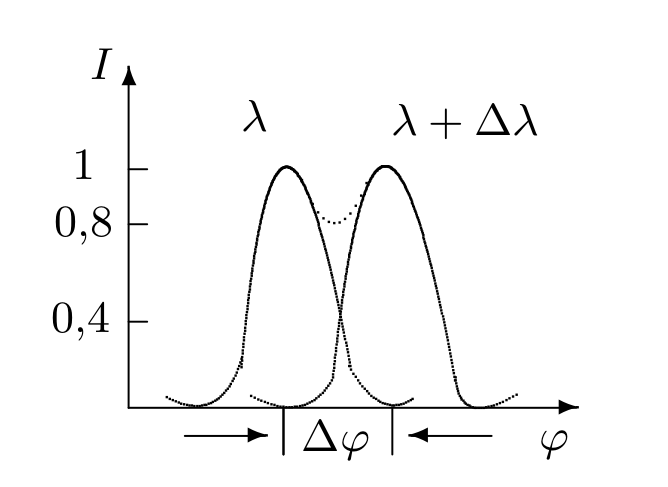
\includegraphics[width = 0.5\linewidth]{k.png}
			\caption{К определению разрешающей способности дифракционной решётки}
		\end{center}
		
	\end{figure}
	Дисперсионная область $G$ "--- предельная ширина спектрального интервала $d \lambda$, при которой спектры соседних порядков перекрываются только своими границами:
\begin{equation}
	G = d \lambda = \frac{\lambda}{m}.
\end{equation}
	
	\textbf{Экспериментальная установка:}
	
	Схема экспериментальной установки приведена на рис. 2. Опыт выполняется с помощью измерительного микроскопа.
	На столик микроскопа помещается держатель с полированной пластинкой из
	чёрного стекла. На пластинке лежит исследуемая линза.
	
	\begin{figure}[H]
		\begin{center}
			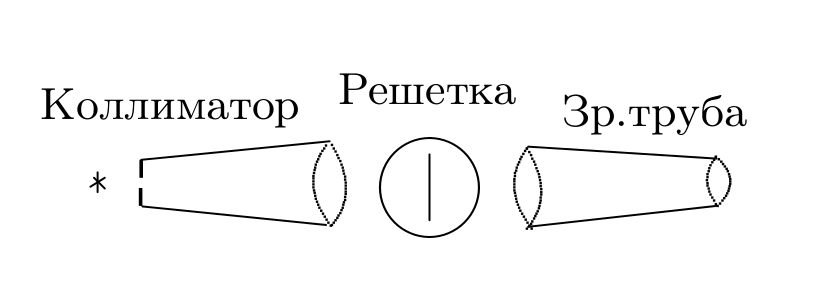
\includegraphics[width=0.6\linewidth]{ust.png}
			\caption{Схема экспериментальной установки (вид сверху)}
		\end{center}
	\end{figure}
	
	ри работе с дифракционной решёткой основной задачей является точное измерение углов, при которых наблюдается главные максимум для различных длин волн.
	Эшелет "--- отражательная решётка с  треугольным профилем штриха, в которой угол $\Omega$ между рабочей гранью и плоскостью решётки не превышает $20^o$
	Рабочий порядок $m \leq 10$, число штрихов $n = 1200\ штр/мм$.
	
	Угол, под которым наблюдается максимум интенсивности функции $I_{1} (\varphi)$, соответствует зеркальному отражению падающего луча от грани и называется углом блеска $\varphi_{б}$.
\begin{equation}
	\varphi_{б} = \psi + 2 \Omega,
\end{equation}
	где $\psi$ "--- угол, под которым падает плоская монохроматическая волна $\lambda$.
	
	Разность хода $\Delta$ кратна $\lambda$:
\begin{equation}
	\Delta = d (\sin \varphi_m - \sin \varphi) = m \lambda.
\end{equation}
	Изменяя угол падения, можно добиться того, чтобы угол блеска совпал с углом дифракции спектра одного из порядков; в этом порядке спектр будет наиболее ярким. Этот порядок принять называть рабочим.
	\begin{figure}[H]
		\begin{center}
		
		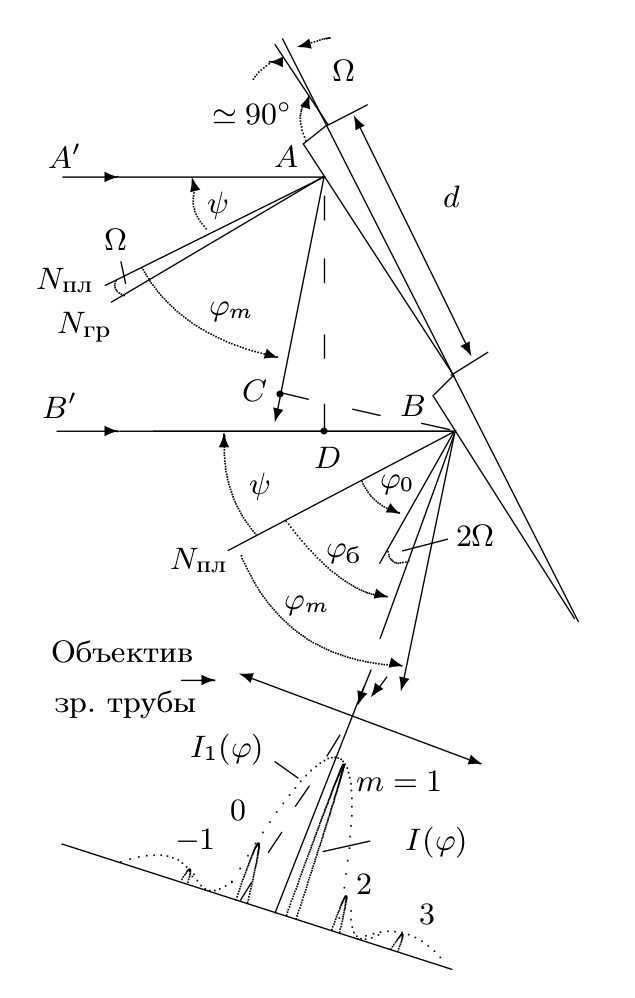
\includegraphics[width = 0.3\linewidth]{3.png}
		\caption{Распределение интенсивности в спектре эшелета}
		\end{center}
	\end{figure}
	
	Чтобы устранить произвол в выборе угла падения, принято считать, что решётка должна работать в автоколлиматорном режиме. В этом случае условие $d(\sin \\varphi_m + \sin \varphi) = m \lambda$ принимает вид:
\begin{equation}
	2d \sin \Omega = m_p \lambda_p.
\end{equation}
	Для оценки $\Delta \varphi_m$ воспользуемся методом векторных диаграмм:
	\begin{figure}[H]
		\begin{center}
		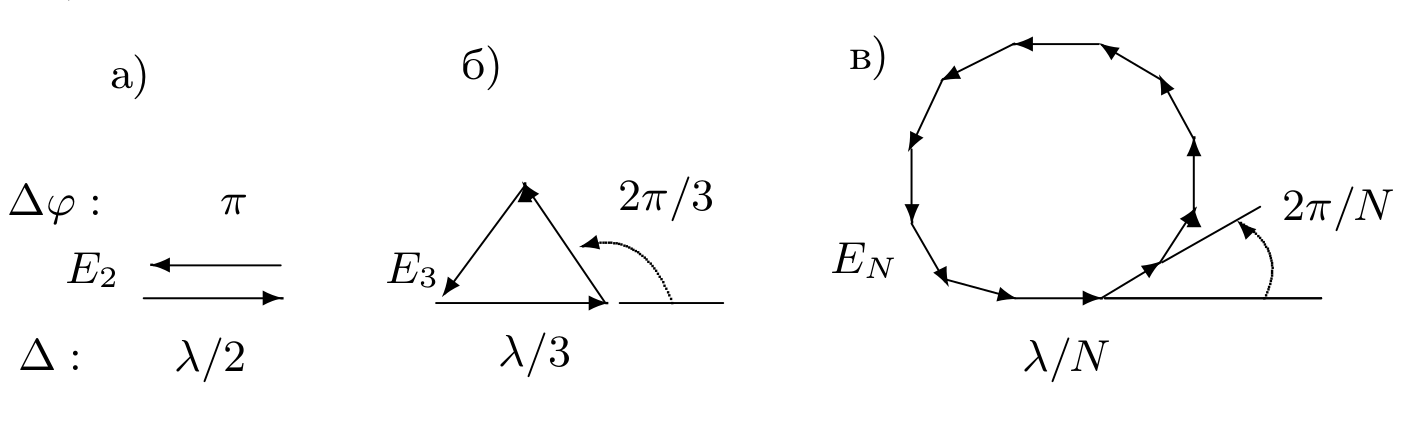
\includegraphics[width = 0.7\linewidth]{2.png}
		\caption{Векторные диаграммы}
	\end{center}
	\end{figure}
	Направление на минимум, ближайший к максимуму любого порядка:
\begin{equation}
	d(\sin(\varphi_m + \Delta \varphi) + \sin \psi) = m \lambda + \frac{\lambda}{N}
\end{equation}
	Для малой полуширины максимума получим:
\begin{equation}
	\Delta \varphi = \frac{\lambda}{Nd\cos \phi_m}
\end{equation}
	Зависимость дисперсии $D$ от параметров эшелета:
\begin{equation}
	D = \frac{m}{d \cos \varphi_m} = \frac{m}{\sqrt{d^2 - (m \lambda - d \sin \psi)^2}}
\end{equation}
	
	\newpage
	
	\textbf{Ход работы и обработка результатов.}\\
	
	
Для угла $\psi = 45^o$ измерим угловые координаты спектральных линий ртути в рабочем порядке. Отметим главную координату каждой из описанных линий:
\begin{table}[H]
	\centering
	\begin{tabular}{|c|c|c|}  \hline
		Ахроматический & $45^o 01' 00''$ & {} \\\hline
		Фиолетовый & $287^o 00' 09''$ & $4047 \dot A$ \\\hline
		Синий & $288^o 20' 09''$ & $4358 \dot A$ \\\hline
		Голубой & $290^o20'09''$ & $4916 \dot A$ \\\hline
		Зелёный & $292^o20'09''$ & $5461 \dot A$ \\\hline
		Желтый 2 & $293^o 30' 09''$ & $5770 \dot A$ \\\hline
		Жёлтый 1 & $293^o 40'09''$ & $5791 \dot A$ \\\hline
		Красный 2 & $294^o 40' 09''$ & $6234 \dot A$ \\\hline
		Красный 1 & $294^o 50'09''$ & $6907 \dot A$ \\\hline
	\end{tabular}
\end{table}
Для оценки разрешающей способности измерим ширину одной из линий жёлтого дублета и рассчитаем аппаратную полуширину линии $\Delta \lambda$:

\begin{equation}
\Delta \lambda = 21; \quad R = \frac{\lambda}{\Delta \lambda} =\frac{5770}{21} =  274.6
\end{equation}
Для угла $\psi = 30^o$ измерим координаты каждой из жёлтых линий во всех наблюдаемых порядках:
\begin{table}[H]
	\begin{center}
		\begin{tabular}{|c|c|c|} \hline
			& $Ж_1$ & $272^o00'07''$ \\
			\cline{2-3}
			$I_{пол}$
			& $Ж_2$ & $272^o 10'07''$ \\\hline
			& $Ж_1$ & $321^o10'09''$ \\
			\cline{2-3}
			$II_{отр}$
			& $Ж_2$ & $321^o10'09''$ \\\hline
		\end{tabular}
	\end{center}
\end{table}
Повторим измерения для $\psi = 45^0, 60^o$:

\begin{table}[H]	
	\begin{center}
		\begin{tabular}{|c|c|c|} \hline
			& $Ж_1$ & $314^o 00'09''$\\
			\cline{2-3}
			$I_{отр}$
			& $Ж_2$ & $313^o30'09''$ \\\hline
			& $Ж_1$ & $293^o40'09''$ \\
			\cline{2-3}
			$II_{отр}$
			& $Ж_2$ & $293^o30'09''$ \\\hline
		\end{tabular}
		\caption{$\psi = 45^o$}
	\end{center}
\end{table}

\begin{table}[H]	
	\begin{center}
		\begin{tabular}{|c|c|c|} \hline
			& $Ж_1$ & $268^o40'09''$\\
			\cline{2-3}
			$I_{отр}$
			& $Ж_2$ & $268^o30'09''$ \\\hline
			& $Ж_1$ & $289^o50'09''$ \\
			\cline{2-3}
			$II_{отр}$
			& $Ж_2$ & $290^o00'09''$ \\\hline
			& $Ж_1$ & $309^o50'09''$\\
			\cline{2-3}
			$III_{отр}$
			& $Ж_2$ & $310^o00'09''$ \\\hline
		\end{tabular}
		\caption{$\psi = 60^o$}
	\end{center}
\end{table}


Построим график зависимости $\sin \varphi_m - sin \psi= f(\lambda)$ и по углу наклона определим период эшелета:
\begin{figure}[H]
	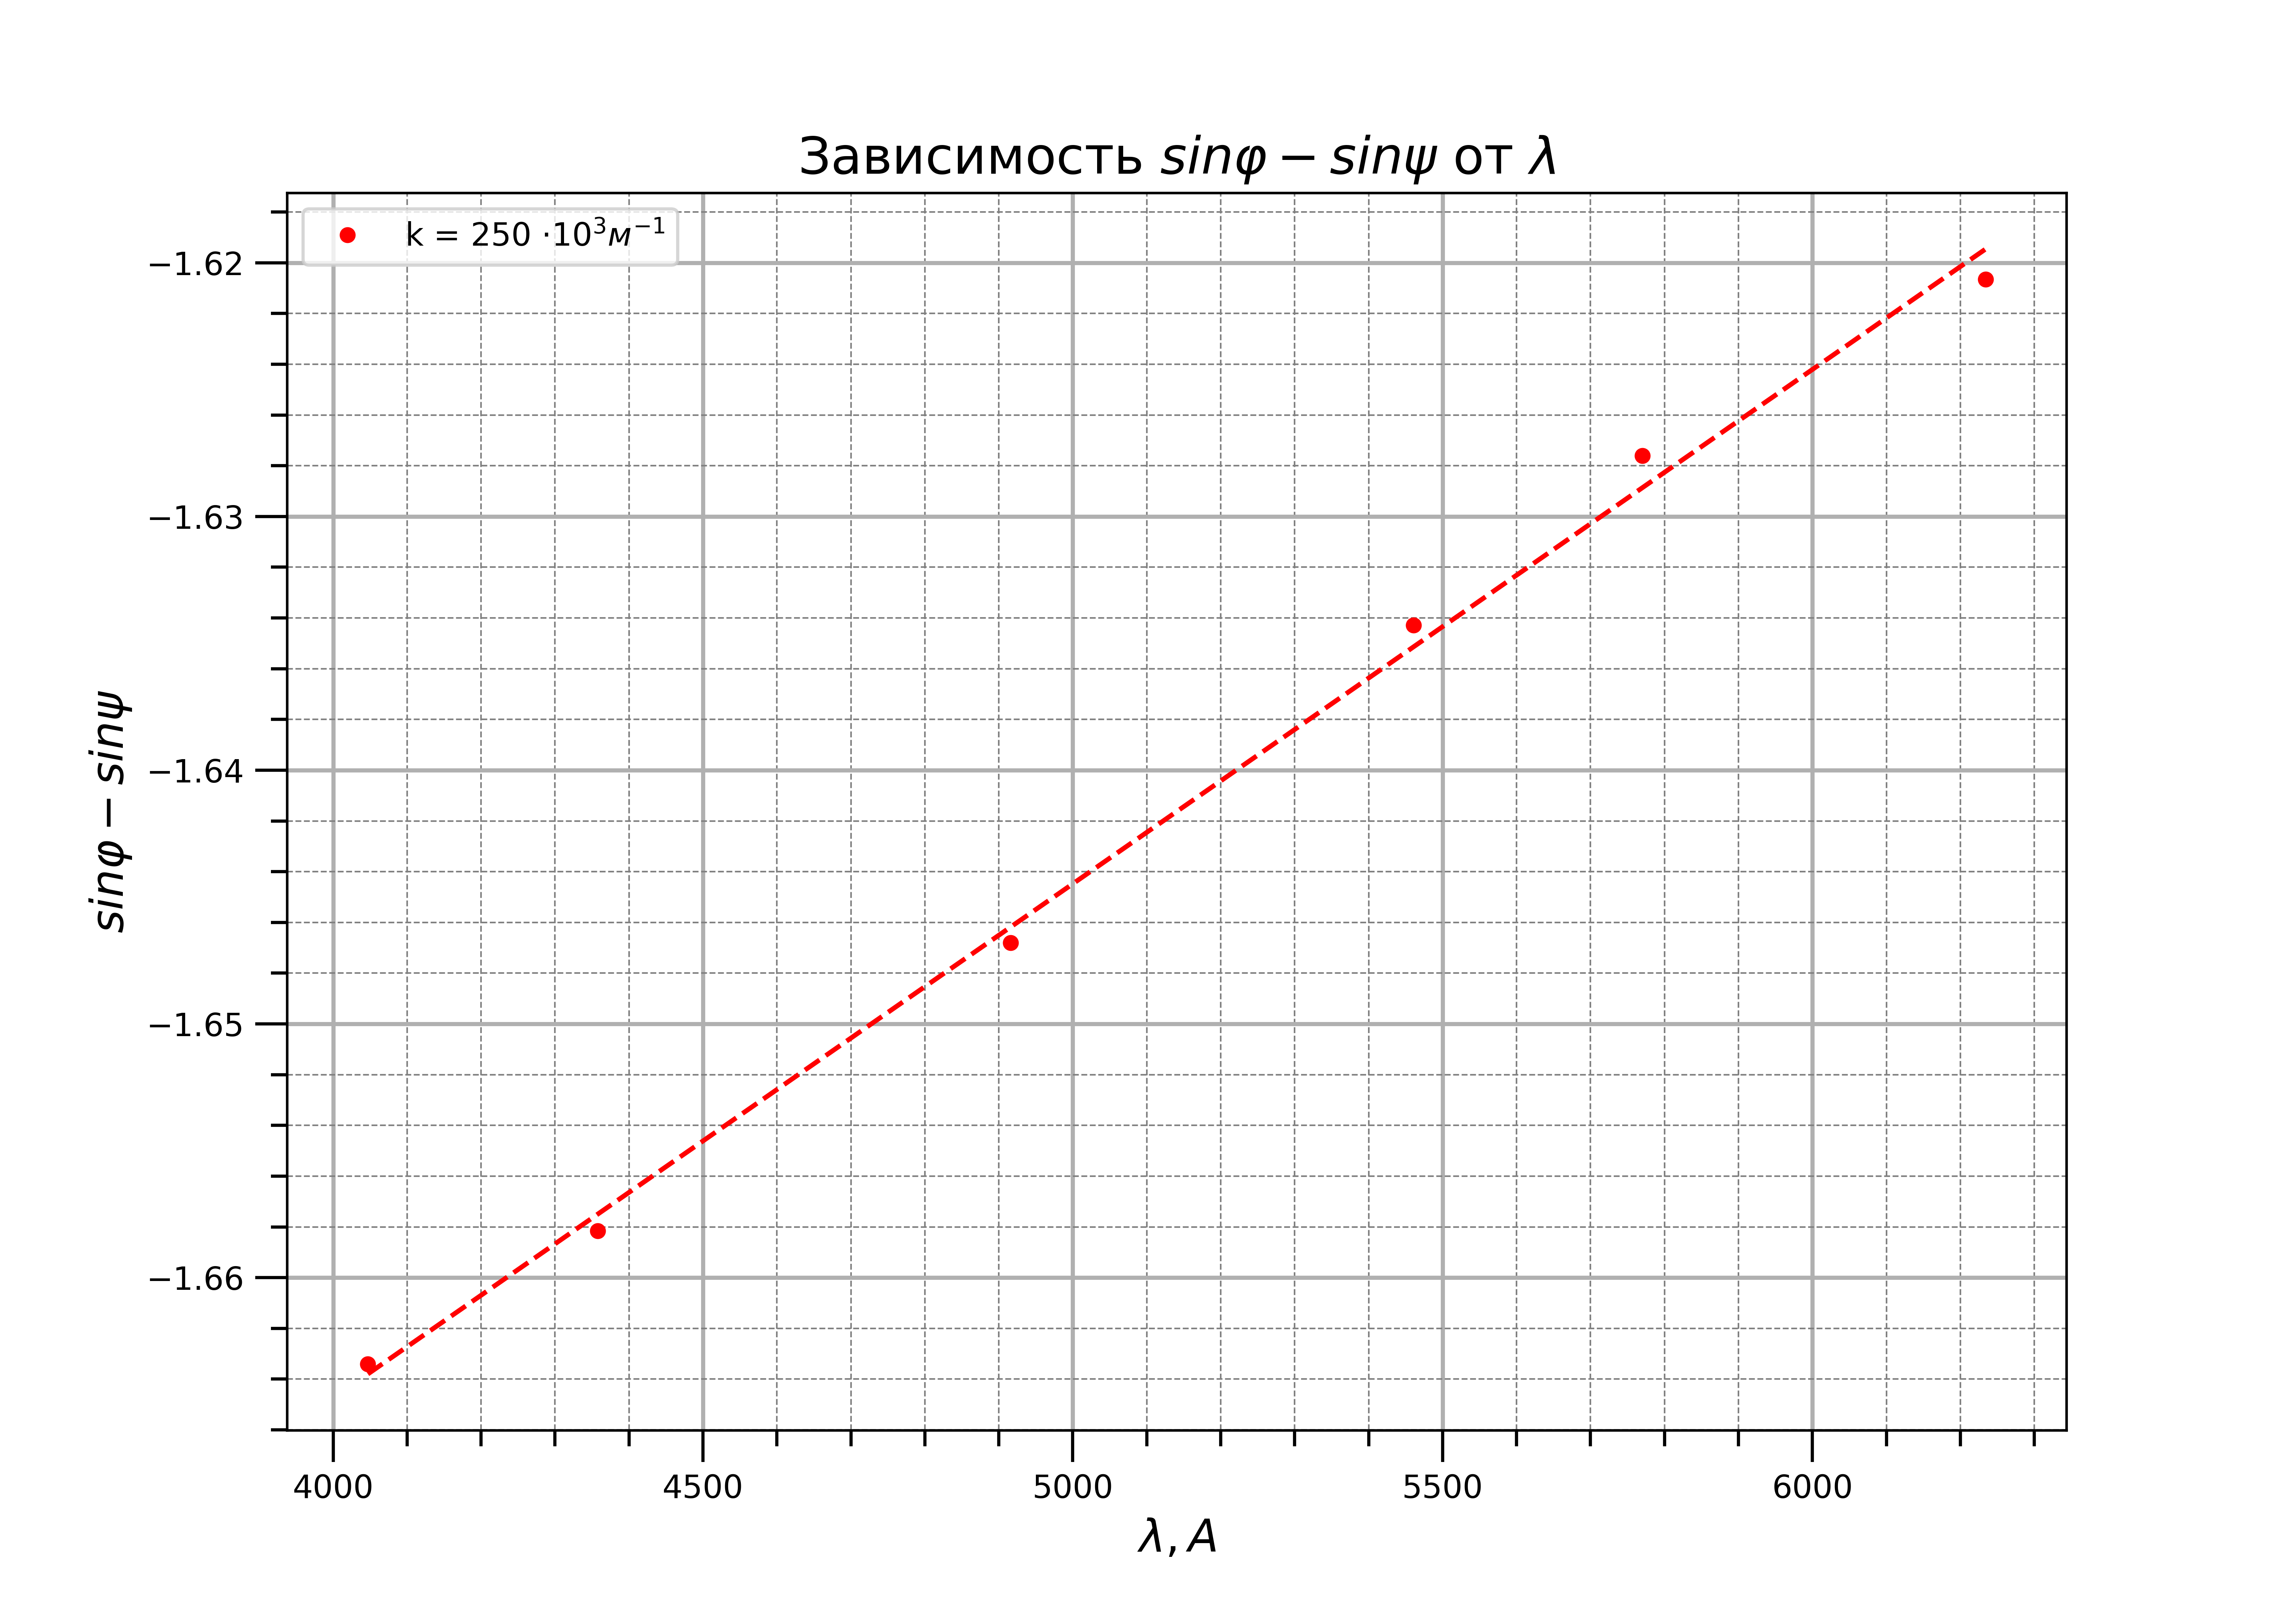
\includegraphics[width = 1.0\linewidth]{sin.png}
	\caption{Зависимость $\sin \varphi_m$ от $\lambda$}
\end{figure}
Угол наклона графика $k = (100 \pm 13)\cdot 10^3$

Период эшелета: $d = \frac{10^{-3}}{100} = (1 \pm 0.2) \cdot 10^{-2}$ мм .

Угол скоса по формуле (15) и $ m_{p} = 1 $, $ \lambda_{р} = 500 $нм, тогда
\begin{equation*}\label{key}
	\sin \Omega = \frac{m_{p} \lambda_{р}}{2 d} = 0.025\pm 0.005
\end{equation*}
\begin{equation*}\label{key}
	\Omega = 1.64^\circ \pm 0.02^\circ.
\end{equation*} 
Угловая дисперсия в рабочем порядке для жёлтого дублета в угловых секундах на $\dot A$:

\begin{table}[H]
	\begin{center}

	\begin{tabular}{|c|c|c|c|}
		\hline
		$\varphi$ &
		$\left|\Delta \varphi\right|$ &
		$\Delta \lambda$, \AA{} &
		$\left|\frac{d \varphi}{d \lambda}\right|_{эксп}$, (угл. с./\AA{}) \\ \hline
		$30^\circ$ & $49\pm 1$  & $21$ & $2.5\pm 0.2$ \\ \hline
		$45^\circ$ & $21\pm 10$ & $21$ & $1\pm 0.1$ \\ \hline
		$60^\circ$ & $21\pm 10$ & $21$ & $1\pm 0.1$ \\ \hline
	\end{tabular}
	\caption{Угловая дисперсия при различных $ \varphi $}
		\end{center}
\end{table}


	

	
	\textbf{Обсуждение результатов и выводы: }\\
	В данной лабораторной работе мы исследовали спектральные характеристики дифракционной решётки, научились работать с гониометром, экспериментально определили период решётки и  разрешающую способность.
	
	
	
\end{document}
